\chapter{Lecture 25: Integrating functions of two variables} \label{double integral}
In section \ref{r(i,j)} we defined our first function of two variables, $r(i,j)$; \textbf{this was a discrete function of two variables}, $i$ (the row corresponding to the week of interest) and $j$ (the column corresponding to the day of interest); its output was the value in position $i,j$ on the table of rainfall data. \\

\noindent Understanding \textbf{continuous functions of two variables} will involve a little bit more explanation and visualisation. For a function of 1 variable, we usually label the input $x$, and we label the output $y$. For functions of 2 variables, we usually label the inputs $x$ and $y$, and we label the output $z$. So instead of $y = f(x)$ we have

  	\bigskip
	
	\hfil\fbox{
	\begin{minipage}{0.18\columnwidth}{
	
	\vskip 0.04cm
	\begin{center}
	$\displaystyle{z = f(x,y)}$
	\end{center}
	}
	\end{minipage}}
	\bigskip
	\bigskip

Both $x$ and $y$ belong to intervals of the real number line. This means we can look at $x$ and $y$ on a coordinate system:
\begin{center}
\begin{tikzpicture}[scale=0.8]
\axesmacro{-0.3}{4}{-0.3}{4}{x}{y}
\draw [fill = black] (2,2) circle (0.04cm) node  [above] {$(x_1,y_1)$};
\draw (2,0) node {\tiny$|$} node [below = 1mm] {$x_1$};
\draw (0,2) node [rotate = 90] {\tiny$|$} node [left = 1mm] {$y_1$};
\end{tikzpicture}
\end{center}
Any input value, $(x,y)$, can be represented on this (flat) coordinate system. This is called a \textbf{plane}. Since it is made of two variables which both belong to $\R$, we call this plane $\R^2$ (sometimes the plane is referred to as `two dimensional'). So, while a continuous function $f(x)$ takes inputs from some interval of $\R$, a continous function $f(x,y)$ takes inputs from a section of $\R^2$. \\

\noindent So, we have a way to visualise the inputs of $f(x,y)$, but how will we visualise the outputs? To do this, we need another axis, the $z$ axis. We need to draw the $z$ axis perpendicular to the $y$ axis and the $x$ axis. The only ways to do this are to draw the $z$-axis pointing into the page, or out of the page. By convention, we draw it pointing out of the page. So that we can visualise it better, we draw an artists interpretation:
\begin{center}
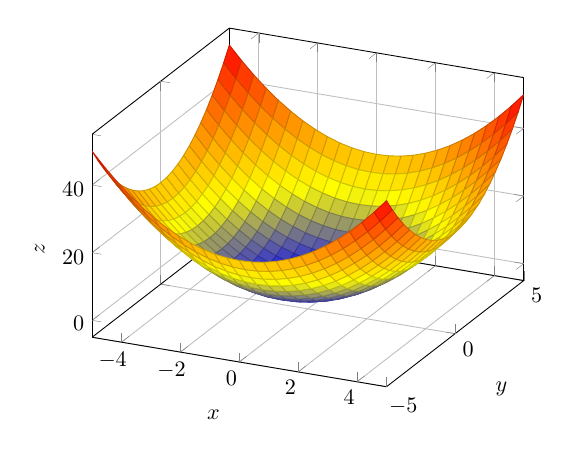
\begin{tikzpicture}[scale=0.8]
\begin{axis}[grid=both,
xlabel={$x$},
ylabel={$y$},
zlabel={$z$}
]
\addplot3[surf,shader=faceted] {(\x)^2 + (\y)^2};
\end{axis}
\end{tikzpicture}
\end{center}
Above is a plot of the function $f(x,y) = x^2 + y^2$, for the section $y \in [-5,5]$ and $x \in [-4,4]$. The $z$-axis points upwards, and has values roughly $z \in [0,40]$. For each input value $(x_1,y_1)$, we colour in the point $z_1$ at the height $z_1 = x_1^2 + y_1^2$ up the $z$-axis; this is what forms the coloured surface. The program used to generate this plot chooses to shade points based on the value of $z$, so points of equal height have the same shade in this picture. \\

\noindent We interpreted the integral of $f(x)$ as the `\textit{area} under the graph' of $f(x)$. As we can see in the above image, the plot of $f(x,y)$ is a \textbf{surface}; we interpret the integral of $f(x,y)$ to be the \textit{volume} under the graph of $f(x,y)$ (i.e., the volume between the coloured surface and the $x,y$-plane). \\

\noindent In section \ref{multiple summation}, we learned how to sum over a function of two variables. We learned that to sum $r(i,j)$ over $i$ and $j$ we write
\[
\sum_i \sum_j r(i,j) 
\] 
Which means that we wish to sum $r(i,j)$ with respect to $j$ first, then sum with respect to $i$. This is actually just finding the \textbf{sum of a sum}. We also learned that we can interchange the order of summation, without changing the meaning. \\

\noindent Integrating with respect to two variables, $x$ and $y$, is just like summing with respect to two variables: It is actually just finding the \textbf{integral of an integral}. We need to integrate with respect to one variable first, then the other variable. When integrating $f(x)$, with respect to $x$, we write $\int_a^b f(x) \; dx$. When integrating $f(x,y)$ with respect to $x$ and $y$, we write

  	\bigskip
	
	\hfil\fbox{
	\begin{minipage}{0.35\columnwidth}{
	
	\vskip 0.04cm
	\begin{center}
	$\displaystyle{\int_c^d \int_a^b f(x,y) \; dx dy}$
	\end{center}
	}
	\end{minipage}}
	\bigskip
	\bigskip

\noindent Which says that we wish to integrate with respect to $x$, from $a$ to $b$, then integrate with respect to $y$, from $c$ to $d$. Just like with summation, we can interchange the order of integration without changing the meaning, so we can write,
\[
\int_c^d \int_a^b f(x,y) \; dx dy = \int_a^b \int_c^d f(x,y) \; dy dx
\]
Which, on the right hand side, says to integrate with respect to $y$ first (from $c$ to $d$), then $x$ (from $a$ to $b$). With some examples you will see that if you know how to integrate with respect to one variable, then you can easily integrate with respect to two variables!

\subsection{Treating one variable as a constant}
Perhaps the trickiest part of integrating $f(x,y)$ with respect to $x$ and $y$, is to remember that when we integrate with respect to $x$ we need to treat $y$ as a constant, and when we integrate with respect to $y$ we need to treat $x$ as a constant. Try completing the following integrals before looking at the solutions: \\

\noindent \textbf{Example 1:} \\
Evaluate
\[
\int_0^2 x^3 + 3y \; dy.
\]
\solution
We integrate with respect to $y$, treating $x$ as a constant:
\begin{align*}
\int_0^2 x^3 + 3y \; dy & = \int_0^2 x^3 \; dy + \int_0^2 3y \; dy  \tag{linearity} \\
	& = x^3\int_0^2 1 \; dy + 3\int_0^2 y \; dy \tag{linearity, since $x^3$ is constant} \\
	& = x^3\squac{y}^2_0 + 3\squac{\frac{y^2}{2}}_0^2 \tag{integral formulas} \\
	& = 2x^3 + 6.
\end{align*}

\noindent \textbf{Example 2:} \\
Evaluate
\[
\int_{-\infty}^2 y\e^{xy} \; dx
\]
\solution
We integrate with respect to $x$, treating $y$ as a constant:
\begin{align*}
\int_{-\infty}^2 y\e^{xy} \; dx & = y\int_{-\infty}^2 \e^{xy} \; dx \tag{linearity, since $y$ is constant} \\
	& = y\squac{\frac{1}{y}\e^{xy}}_{-\infty}^2 \; dx \tag{since $\int \e^{ax} \; dx = \frac{1}{a}\e^{ax}$} \\
	& = y\brac{\frac{1}{y}\e^{2y} - 0} \tag{since $\e^{ax} \rightarrow 0$ as $x \rightarrow -\infty$} \\
	& = \e^{2y}.
\end{align*}

\noindent Notice that when we evaluate a definite integral with respect to $y$, the resulting expression does not depend on $y$, and when we do so with respect to $x$, the resulting expression does not depend on $x$. This should always be the case (it is a good sanity check to make sure you haven't made a mistake).

\subsection{Doing multiple integration}
We will now learn how to evaluate double integrals by going through some examples. Try to do as many of the examples as you can before looking at the solutions. \\

\noindent \textbf{Example 1:} \\
Evaluate
\[
\int_1^2 \int_0^1 (4-x-y) \; dx dy
\]
\solution
We must evaluate the `inside' integral first, that is, we integrate with respect to $x$ first, from $0$ to $1$, treating $y$ as a constant:
\begin{align*}
\int_0^1 (4-x-y) \; dx & = 4\int_0^1 1 \;dx - \int_0^1 x \; dx - y\int_0^1 1 \; dx \tag{linearity, $y$ is constant} \\
	& =  4\squac{x}^1_0 - \squac{\frac{x^2}{2}}^1_0 - y\squac{x}^1_0 \tag{integral formulas} \\
	& = \frac{7}{2} - y.
\end{align*}
So far, by evaluating the `inner' integral, we have found that
\[
\int_1^2 \int_0^1 (4-x-y) \; dx dy = \int_1^2 \frac{7}{2} - y \; dy.
\]
Now we must integrate with respect to $y$:
\begin{align*}
 \int_1^2 \frac{7}{2} - y \; dy & = \frac{7}{2}\int_1^2 1 \; dy - \int_1^2 y \; dy \tag{linearity} \\
 	& = \frac{7}{2}\squac{y}_1^2 - \squac{\frac{y^2}{2}}_1^2 \tag{integral formulas} \\
 	& = 7 - \frac{7}{2} - 2 + \frac{1}{2} \\
 	& = 2.
\end{align*}
We evaluated the `inner' integral, then evaluated the `outer' integral, and we found that
\[
\int_1^2 \int_0^1 (4-x-y) \; dx dy = 2.
\]
It is a good exercise to interchange the order of integration and check that you get the same result. Interchanging gives
\[
\int_0^1 \int_1^2 (4-x-y) \; dy dx.
\]
Evaluate this as an exercise, and check that the result is equal to $2$.
\bigskip

\noindent \textbf{Example 2:} \\
In lecture 27, we will learn about `joint probability density functions;' these are functions, $f(x,y)$, of two variables, whose outputs are probabilities. We claim that the following function is a joint pdf 
\[
f(x,y) = \left\{ \begin{array}{ll}
\frac{2}{3}(x + 2y), & \; \text{if} \;\; 0 \leq x \leq 1 \; \text{and} \; 0 \leq y \leq 1 \smallskip \\
0, & \; \text{otherwise}
\end{array} \right.
\]
Check that this function satisfies probability measure axiom 1; i.e., check that the integral over all possible values of $x$ and $y$ is equal to 1. \\

\solution
Since the only values of $x$ and $y$ for which $f(x,y) \neq 0$ are $x \in [0,1]$ and $y \in [0,1]$, we wish to find
\[
\int_0^1 \int_0^1 \frac{2}{3}(x + 2y) \; dxdy
\]
We evaluate the `inner' integral first (this time we will save space by doing it in square brackets):
\begin{align*}
\int_0^1 \squac{\int_0^1 \frac{2}{3}(x + 2y) \; dx} dy & = \int_0^1 \squac{\int_0^1 \frac{2}{3}x + \frac{4}{3}y \; dx} dy \tag{expanding brackets} \\
	& = \int_0^1 \squac{\frac{2}{3}\squac{\frac{x^2}{2}}_0^1 + \frac{4}{3}y\squac{x}_0^1} dy \tag{$y$ is constant} \\
	& = \int_0^1  \squac{\frac{1}{3} + \frac{4}{3}y} \; dy \tag{now evaluate `outer' integral} \\
	& = \frac{1}{3}\squac{y}^1_0 + \frac{4}{3}\squac{\frac{y^2}{2}}^1_0 \\
	& = 1.
\end{align*} 
Which is what we wanted to show. 


\subsection{Decouple double integrals with product structure} \label{decouple} \label{product structure}
There is one more useful property of double integrals that we need to cover. This property is called \textbf{decoupling}, and it only applies when $f(x,y)$ can be expressed as a product of two functions. If $f(x,y) = h(x)g(y)$, for some functions $h$ and $g$, then $f(x,y)$ is referred to as having \textbf{the product structure}, and

  	\bigskip
	
	\hfil\fbox{
	\begin{minipage}{0.55\columnwidth}{
	
	\vskip 0.04cm
	\begin{center}
	$\displaystyle{\int_c^d \int_a^b f(x,y) \; dx dy = \int_a^b h(x) \; dx\int_c^d \! g(y) \;dy}$
	\end{center}
	}
	\end{minipage}}
	\bigskip
	\bigskip

\noindent In the next section, where we integrate the Gaussian, we will use this property (going from right to left) with the case $h(x)g(y)  = \e^{-x^2}\e^{-y^2} = \e^{-(x^2+y^2)} = f(x,y)$. \\

\noindent Some other functions which have the product structure are
\begin{itemize}
\item $f(x,y) = xy, \;\;\;\;\;\;\;\; \text{where $h(x) = x$ and $g(y) = y$}$
\item $f(x,y) = x^3(3-y^2), \;\;\;\;\;\;\;\; \text{where $h(x) = x^3$ and $g(y) = 3-y^2$}$
\end{itemize}

\noindent Some functions which do not have the product structure are
\begin{itemize}
\item $f(x,y) = x + y$
\item $f(x,y) = x^y$
\end{itemize}
When $f(x,y)$ does \textit{not} have the product structure, the integrals do \textit{not} decouple.

\section{Integral of the Gaussian (difficult)}
In section \ref{bell curve} we introduced the Gaussian function $f(x) = \e^{-x^2}$, then in section \ref{normal distribution} we introduced the pdf of the normal distribution, which is a variation of the Gaussian function. Now, we finally have the tools to find
\[
\int_{-\infty}^\infty \e^{-x^2} \; dx
\]
Evaluating this integral is not particularly easy, and the solution presented here is due to Carl Friedrich Gauss. Students who are new to the ideas in this course may have trouble following along. We start by recognising that $\e^{-x^2}$ has even symmetry, so
\[
\int_{-\infty}^\infty \e^{-x^2} \; dx = 2\int_0^\infty \e^{-x^2} \; dx.
\]
Now, the trick is to start off by squaring this integral. Notice that $x$ is just a dummy variable, so we can write
\begin{align*}
\brac{\int_0^\infty \e^{-x^2} \; dx}^2 & = \int_0^\infty \e^{-x^2} \; dx \int_0^\infty \e^{-y^2} \; dy  \tag{replacing $x$ with $y$}\\
		& = \int_0^\infty \int_0^\infty \e^{-x^2}\e^{-y^2} \; dxdy \tag{product structure, section \ref{decouple}} \\
		& =  \int_0^\infty \int_0^\infty \e^{-(x^2 + y^2)} \; dxdy \tag{index laws}
\end{align*}
Now we make a (right-to-left) substitution $y = xt$, so $\frac{dy}{dt} = \frac{d}{dt}(xt) = x$, and the terminals remain the same. So
\begin{align*}
\brac{\int_0^\infty \e^{-x^2} \; dx}^2 & = \int_0^\infty \int_0^\infty \e^{-(x^2 + (xt)^2)} \; x dxdt \tag{integration by substitution} \\
	& = \int_0^\infty \int_0^\infty \e^{-(1 + t^2)x^2} \; x dxdt \tag{factoring out $x^2$}
\end{align*}
Now we make a second (this time left-to-right) substitution $u = x^2$, so $\frac{du}{dx} = 2x$, so $x = \frac{1}{2}\frac{du}{dx}$, and the terminals again remain the same.
\begin{align*}
\brac{\int_0^\infty \e^{-x^2} \; dx}^2 & = \frac{1}{2}\int_0^\infty \squac{ \int_0^\infty \e^{-(1 + t^2)u} \; du} dt \tag{substitution again} \\
	& = \frac{1}{2}\int_0^\infty \squac{ \squac{-\frac{1}{1+t^2} \e^{-(1 + t^2)u}}_0^\infty } dt \tag{$-(1+t^2)$ is constant} \\
	& =  \frac{1}{2}\int_0^\infty \frac{1}{1+t^2} \; dt \tag{since $\e^{-(1+t^2)u} \rightarrow 0$ as $u \rightarrow \infty$} \\
	& = \frac{1}{2}\squac{\arctan(t)}_0^\infty \tag{trig substitution, outside scope of this course} \\
	& = \frac{\pi}{4} \tag{$\arctan$ is outside the scope of this course}
\end{align*}
For those who understand the arctan function, note that $\arctan(t) \rightarrow \pi/2$ as $t \rightarrow \infty$, and that $\arctan(0) = 0$, which justify the previous step. \\

\noindent So far we have,
\[
\brac{\int_0^\infty \e^{-x^2} \; dx}^2 = \frac{\pi}{4}.
\]
Taking the square root of both sides gives
\[
\int_0^\infty \e^{-x^2} \; dx = \frac{\sqrt{\pi}}{2}.
\]
Recall that the integral we want is twice this, so:
\[
\int_{-\infty}^\infty \e^{-x^2} \; dx = 2\brac{\int_0^\infty \e^{-x^2} \; dx} = 2\brac{ \frac{\sqrt{\pi}}{2}} =  \sqrt{\pi}.
\]

\subsection{Check validity of pmf of normal distribution} \label{check normal distribution}
Recall that the pmf of the normal distribution is
\[
f(x) = \frac{1}{\sigma \sqrt{2\pi}} \exp\brac{-\frac{(x-\mu)^2}{2\sigma^2}}
\]
We can check probability measure axiom 1 for this pmf, using the result above for the integral of the Gaussian. We have,
\[
\int_{-\infty}^\infty \e^{-x^2} \; dx = \sqrt{\pi}.
\]
Now, we define $x = \frac{z-\mu}{\sigma\sqrt{2}}$. Rearranging for $z$ gives $z = \sigma\sqrt{2} x + \mu$. So $\frac{dz}{dx} = \sigma\sqrt{2}$. Thus $\frac{1}{\sigma\sqrt{2}}\frac{dz}{dx} = 1$. In the next step we multiply the above integral by $\frac{1}{\sigma\sqrt{2}}\frac{dz}{dx}$, which, we have just seen, is equal to $1$. Hence,
\[
\frac{1}{\sigma\sqrt{2}} \int_{-\infty}^\infty \e^{-x^2} \; \frac{dz}{dx} dx = \sqrt{\pi}
\]
We defined $x = \frac{z-\mu}{\sigma\sqrt{2}}$. Notice that $z \rightarrow \pm\infty$ as $x \rightarrow \pm\infty$. Thus, using left-to-right substitution, the terminals will remain the same:
\[
\frac{1}{\sigma\sqrt{2}} \int_{-\infty}^\infty \exp\brac{-\bfrac{z-\mu}{\sigma\sqrt{2}}^2} \; dz = \sqrt{\pi}
\]
Dividing both sides by $\sqrt{\pi}$, and simplifying gives
\[
\frac{1}{\sigma\sqrt{2\pi}} \int_{-\infty}^\infty \exp\brac{-\frac{(z-\mu)^2}{2\sigma^2}} \; dz = 1.
\]
Which is what we wanted to show.

\subsection{Checking that $\boldsymbol{\Gamma\brac{\frac{1}{2}} = \sqrt{\pi}}$} \label{gamma1/2 = sqrt(pi)}
We can also use this integral of the Gaussian to prove that $\Gamma\brac{\frac{1}{2}} = \sqrt{\pi}$. In section \ref{gamma function} we defined the gamma function to be
\[
\Gamma(\alpha) = \int_0^\infty x^{\alpha-1}\e^{-x} \; dx
\] 
So, letting $\alpha = \frac{1}{2}$,
\[
\Gamma\bfrac{1}{2} = \int_0^\infty x^{-\frac{1}{2}}\e^{-x} \; dx \tag{$\bigstar$}
\]
\bigskip

\noindent Now, recall that $\e^{-x^2}$ is an even function, so the integral of the Gaussian was
\[
2\int_0^\infty \e^{-x^2} \; dx = \sqrt{\pi}.
\]
Defining $u = x^2$, we get $\frac{du}{dx} = 2x$, so $1 = \frac{1}{2x}\frac{du}{dx}$. Hence, in the next step, we are just multiplying the above integral by 1:
\[
2\int_0^\infty \e^{-x^2} \frac{1}{2x} \; \frac{du}{dx} dx = \sqrt{\pi}.
\]
We defined $u = x^2$, thus $x = \sqrt{u}$. Notice that $u = 0$ when $x = 0$ and $u \rightarrow \infty$ as $x \rightarrow \infty$, so the terminals remain the same when we do left-to-right substitution, giving
\[
2\int_0^\infty \e^{-u} \frac{1}{2\sqrt{u}} \; du = \sqrt{\pi}.
\] 
Cancelling the $2$, and writing $\frac{1}{\sqrt{u}} = u^{-\frac{1}{2}}$, we get
\[
\int_0^\infty u^{-\frac{1}{2}} \e^{-u} \; du = \sqrt{\pi}.
\]
On the left hand side we have $\Gamma\bfrac{1}{2}$, from $\bigstar$ (where the dummy variable, $u$, is replaced by $x$), so,
\[
\Gamma\bfrac{1}{2} = \sqrt{\pi}, \;\;\;\; \text{as required.}
\]
